\subsection{Squat wall}

The concrete shear wall being tested in this example is WhittakerSW5 which is 39.6 inches tall (one-story) and 120 inches wide. 
The specimen was tested under cyclic-static action. 
In SWIM, the wall is simulated using 4-node quad plane stress elements. 
Nodes at the bottom are fixed and cyclic displacements are applied to nodes at the top. 
Self weight is distributed to each node as vertical load.
The simulated results are compared with the experiment in \Cref{fig:WhittSW5}.



\begin{figure}[!htbp]
  \centering {
    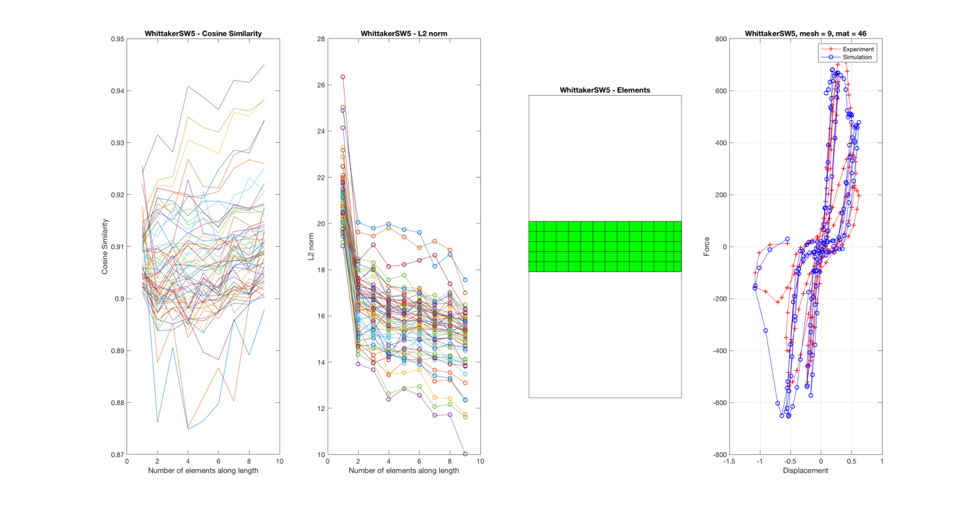
\includegraphics[width=0.95\textwidth]
    {figures/SWIM_WhittSW5.png} }
  \caption{WhittakerSW5}
  \label{fig:WhittSW5}
\end{figure}




\subsection{Tall wall}

The concrete shear wall being tested in this example is OesterleB3 which is 176 inches tall (4 stories) and 75 inches wide. 
The specimen was tested under cyclic-static action. 
In SWIM, the wall is simulated using 4-node quad plane stress elements. 
Nodes at the bottom are fixed and cyclic displacements are applied to nodes at the top. 
Self weight is distributed to each node as vertical load.
The simulated results are compared with the experiment in \Cref{fig:OesterleB3}.


\begin{figure}[!htbp]
  \centering {
    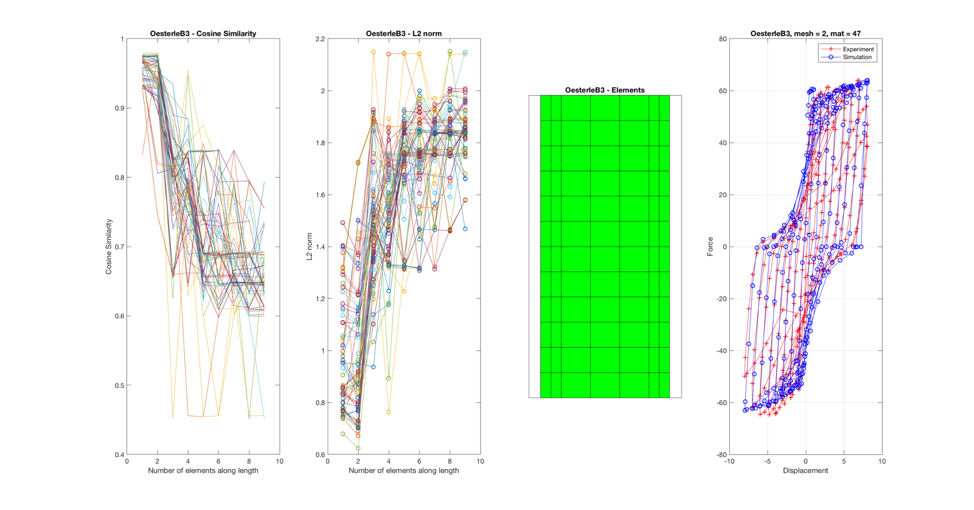
\includegraphics[width=0.95\textwidth]
    {figures/SWIM_OB3.png} }
  \caption{OesterleB3}
  \label{fig:OesterleB3}
\end{figure}

